\chapter{Large Spatial and Temporal Variations of Temperature}
\section{Introduction}
Many different engineering materials are subject to intense heating and cooling in localised regions. As with our previous discussion about materials, the temperature might be spatially or temporally variable. In Lecture 13, we looked at the thermoelastic response of materials subject to small temperature variations. Their response can be dealt with via a linear elastic model. In this chapter, we look at the effect of a large temperature applied to a material which are sufficient to generate a plastic response and how the spatial and temporal variation affects the material properties.

The incandescent light build initially failed due to the thermal fatigue and melting problems. This was largely a material selection and corrosion problem. Turning a light on and off generates enormous thermal stresses, but keeping it on continuously is fine. The filament is made of tungsten which has a high melting point. The inert gases around the filament stop evaporation. Most of energy dissipated is thermal.
\subsubsection{Types of heating processes}
\begin{itemize}
    \item \textbf{Mechanical heating}, usually by friction
    \item \textbf{Electrical heating}, using the material itself for energy release (e.g. induction heating), or more commonly by external means with an electrical resistance made of Nichrome (60\% Ni, 25\% Fe, 15\% Cr) or Kanthal (70\%, 24\% Cr, 5\% Al)
    \item \textbf{Radiation heating}, either with microwaves, infrared radiation from heated wires protected inside a quartz-glass (wires can be made of tungsten, carbon, Kanthal or Nichrome; naked Nichrome coiled wire was also used in the past), or using visible radiation (with a laser).
    \item \textbf{Chemical heating}, mainly by combustion, but also by hydrogen formation after atomic hydrogen is produced in an electric car, for instance.
    \item \textbf{Nuclear heating}, by nuclear fission or fusion
\end{itemize}
\begin{figure}[H]
    \centering
    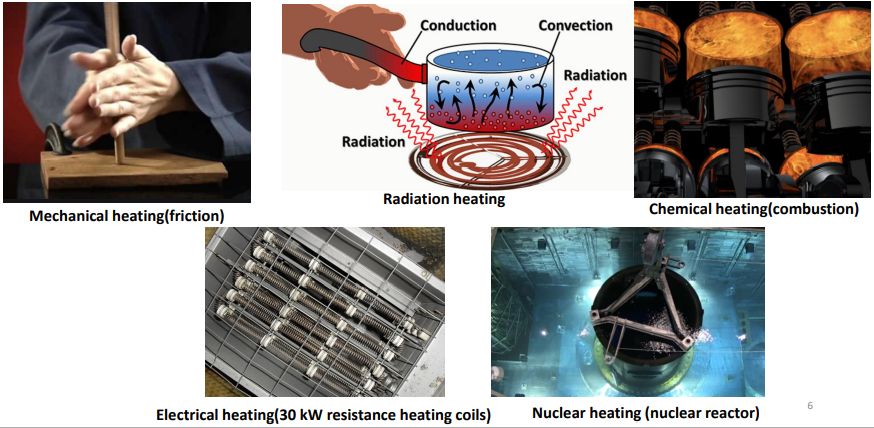
\includegraphics[width = 0.8\textwidth]{img/figure41.png}
    \caption{Heating processes.}
\end{figure}
\begin{figure}[H]
    \centering
    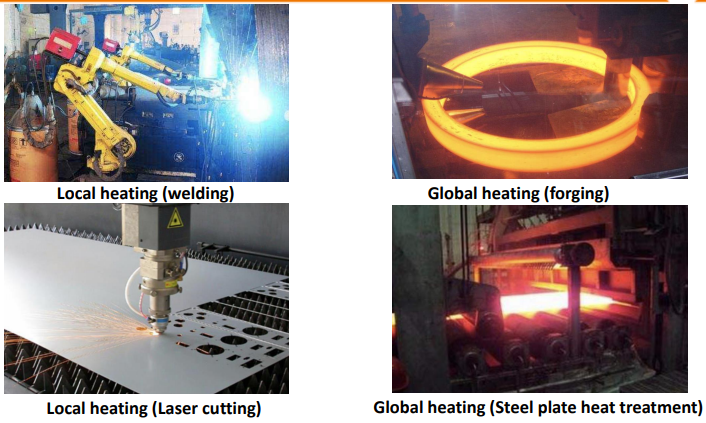
\includegraphics[width = 0.8\textwidth]{img/figure40.png}
    \caption{Localised heating processes.}
\end{figure}
\section{Practical application of heat to a material}
Any time a material is heated, the heat is applied spatially and temporally. The characteristics scales have quite different effects on the material and structure.
\begin{table}[H]
    \centering
    \begin{tabular}{@{}lll@{}}
        \toprule
             & \textbf{Localised} & \textbf{Uniform} \\
        \midrule
        Slow & Welding            & Heat treatment   \\
        Fast & Thermal shocking   & Quenching        \\
        \bottomrule
    \end{tabular}
    \caption{Spatial and temporal heat application.}
\end{table}
\subsection{Welding}
\begin{itemize}
    \item TIG - Tungsten gas - electrode is tungsten. You do not need a metal filter. Need a gas tank to protect the weld - most often applied to stainless steels and light metals
    \item Flux-cored Arc Welding - similar to MIG. Uses a wire to serve as an electrode and a metal filler fed through the wand. Wire has a flux that creates the gas shield. Tends to have slag left so usually needs a clean-up
    \item Stick (Shielded Metal Arc Welding). Replaceable electrode stick t hat forms the filler metal. Arc is created at the end of the electrode. Stick is coated in flux that protects the metal from oxidation
    \item MIG welding (metal inert gas). Filler metal is consumable wire that acts as an electrode
    \item Laser beam welding - used on a few metals with laser providing the heat
    \item Plasma Arc Welding - uses a smaller arc with a high pressurised gas that is ionised and electrically conductive
\end{itemize}
Small amount of molten metal are introduced in the gap between two components to solidify the body. Major regions are:
\begin{enumerate}
    \item Fusion where the parts of the metal have melted and combined with filler material
    \item Heat affected zone - region next to steel that have undergone microstructural changes
\end{enumerate}
\subsection{Friction welding}
\url{https://www.youtube.com/watch?v=RTEP9QdTn5k}
\begin{figure}[H]
    \centering
    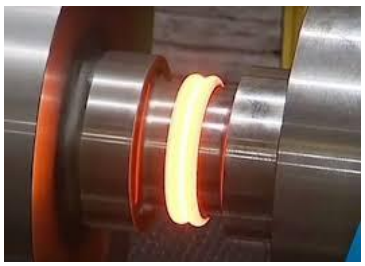
\includegraphics[width = 0.8\textwidth]{img/figure44.png}
    \caption{Friction welding.}
\end{figure}
\subsection{Radiation heating}
\begin{figure}[H]
    \centering
    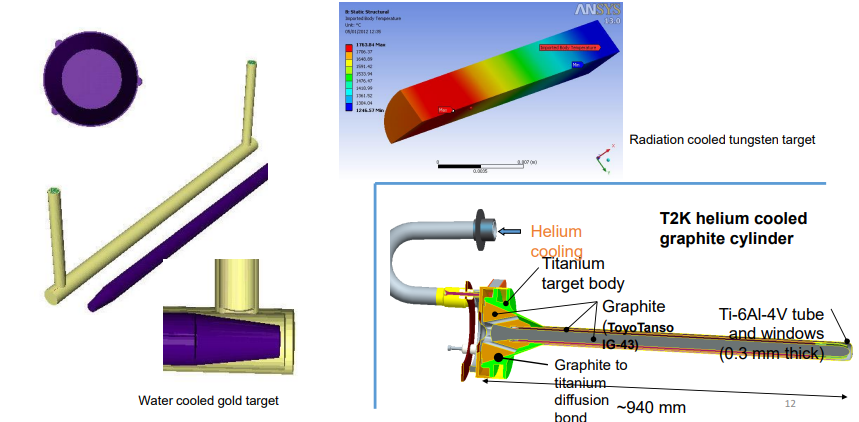
\includegraphics[width = 0.8\textwidth]{img/figure42.png}
    \caption{Radiation heating.}
\end{figure}
\subsection{Laser heating}
\begin{figure}[H]
    \centering
    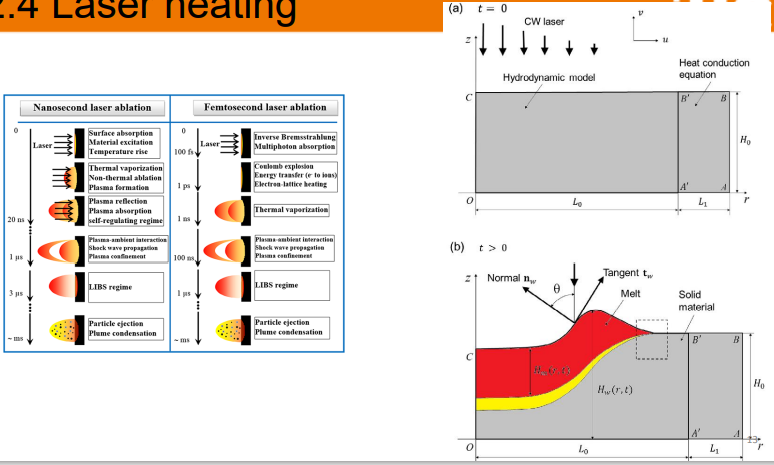
\includegraphics[width = 0.8\textwidth]{img/figure45.png}
    \caption{Laser heating.}
\end{figure}
\begin{figure}[H]
    \centering
    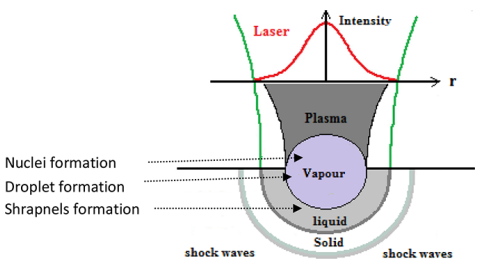
\includegraphics[width = 0.8\textwidth]{img/figure46.png}
    \caption{Close-up of laser heating.}
\end{figure}
\begin{figure}[H]
    \centering
    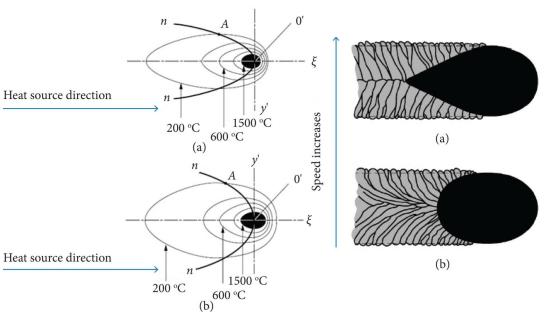
\includegraphics[width = 0.8\textwidth]{img/figure47.png}
    \caption{Close-up of laser heating.}
\end{figure}
The heat spreads out through diffusion from a moving source. The temperature distribution can be analysed using simple mathematical models of a moving source and this is discussed in Worksheet 15.
\section{Structural changes in the matter}
\url{https://www.youtube.com/watch?v=uG35D_euM-0&authuser=0}
\subsection{Microstructural changes}
Metals are comprised of a symmetrical structure of atoms known as an allotrope. Heating the metal will displace atoms from their position and the displaced atoms form a new structure. This process is known as allotropic phase transformation. Allotropic phase transformation alters the hardness, strength and ductility of the metal. The most important allotropic phase transformation is undergone by iron. When iron is heated past \SI{912}{\degree C} it is able to absorb more carbon which is essential for the manufacture of stainless steel.
\begin{figure}[H]
    \centering
    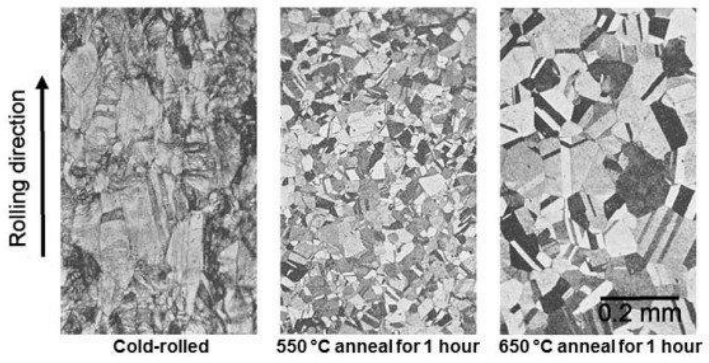
\includegraphics[width = 0.8\textwidth]{img/figure43.png}
    \caption{Effect on microstructure from cold rolling and then annealing.}
\end{figure}
\subsubsection{Heat treatment}
\textbf{Annealing} is used to soften metals including iron, steel, copper, brass and silver. The process involves heating the metal to a specific temperature then allowing it to cool slowly at a controlled rate. Annealing alters the physical and chemical properties of the metal to increase ductility and reduce hardness. This facilitates shaping, stamping or forming processes, and allows the metal to be cut more easily. Annealing also enhances electrical conductivity.

\textbf{Normalising} is applied to alloys to provide uniformity in grain size and composition. The metal is heated to a predefined temperature then cooled by air. The resulting metal is free of undesirable impurities and exhibits greater strength and hardness. Normalising is often used to produce a harder and stronger steel, albeit one that is less ductile than that produced by annealing. Typically, the normalising process is performed on materials that will be subjected to machining, because the process has improved this attribute.

\textbf{Hardening} is applied to steel and other alloys to improve their mechanical properties. During hardening, the metal is heated at a high temperature and this temperature is maintained until a proportion of carbon has been dissolved. Next the metal will is quenched, which involves rapidly cooling it in oil or water. Hardening will produce an alloy which has high strength and and wear resistance. However, hardening will also increase brittleness and is not suitable for engineering applications. When there is a need to have the surface of the component hard enough to resist wear and erosion, while maintaining ductility and toughness to withstand impact and shock loading - surface hardening would be used.

\textbf{Tempering} is applied to steel where ductility is desired. Untempered steel is very hard but too brittle for most practical applications. Tempering is a low temperature heat treatment process normally performed after hardening (neutral hardening, double hardening, atmospheric carburising, carbonitriding, or induction hardening) in order to reach a desired hardness/toughness ratio. the process involves heating steel to a lower temperature to reduce some of the excess hardness. The metal is then allowed to cool in still air which results in a tougher and less brittle steel.
\subsection{Macroscopic changes}
Large temperature variations lead to inelastic and non-recoverable deformations. For plastic deformation require about 0.2\% residual strain. Since the strain generated a temperature difference of $\Delta T$ scales as $\epsilon \sim \Delta T \alpha$. With a typical value of a $\alpha \sim \SI{1e-5}{\per\kelvin}$, we only need $\Delta T \sim \SI{200}{\kelvin}$ to generate this strain. Large temperatures leads to melting, rearrangement of bonds and this is what is used in casting and welding. Ductile and malleable materials can absorb changes while brittle materials fracture.
\section{Soldering, brazing, welding}
\begin{itemize}
    \item Soldering is a low-temperature process (60-\SI{400}{\degree C}) that uses a low-melting metal (a base of tin combined with lead, silver, antimony, bismuth, indium) to join similar or dissimilar metals; it is mainly used in electronic boards
    \item Brazing is a mid-temperature process (450-\SI{1200}{\degree C}) that uses a high-melting metal (a base of silver combined with nickel, copper, zinc) to join similar or dissimilar metals; it is mainly used in copper piping and jewellery
    \item Welding is a high temperature process (800-\SI{2000}{\degree C}) that uses a powerful heat source to locally melt and join similar metals; it is mainly used in iron and steel work
\end{itemize}